%========================================
\chapter{Architectural Description}
%========================================
This chapter introduces the final architectural documents for the project. The team followed the definition of software architecture defined by Len Bass, Paul Clements and Rick Kazman: ``The software architecture of a program or computing
system is the structure of structures of the system, which comprise software elements, the externally visible properties of those elements, and the relationships between them.''~\cite[p.3]{Bass2003}

The purpose of this document is to describe our architecture in a structured way so that it can be used, not only by the team, but also as an aid for other stakeholders who are trying to understand the system.

%-------------------------------------
\section{Architectural Drivers}
%-------------------------------------
This section is dedicated to the discussion of the architectural drivers that were discovered during the project.
The team chose Modifiability and Testability as quality attributes, but it later on became apparent that some care should also be taken considering Performance.

The reason for choosing Modifiability was that the development team would be unable to update or maintain the \gls{utility} after completing this project. The code would also be distributed under a GPL which allows other developers to continue working on the utility and use it for their own applications in the future. It was therefore important that the code would be easy to understand, well documented and easy to modify. Not only will this promote the further development of the utility, but it would also make it easier for the customer to use and modify for their own purposes.

Testability would also be an important quality attribute as the \gls{utility} was to be used by the customer for debugging purposes. It was therefore be very important that the utility it self contained as few bugs as possible so that the customer could be sure that the output given by the utility would be able to help them in analyzing and debugging. The developers of this project were also unable to test any given \glspl{dissector} in a real environment, which made it even more necessary for the developers to do extensive testing of the utility's functionality. This was to ensure that the final product works properly even without the developers having had taken a good look on the data the utility will have to process after going public.

Performance became somewhat of an issue for the utility during the project as it became apparent that the customer would have to run the utility on several thousand header files at once. It would therefore be important for the utility to be able to run through all of the customer's header files in a reasonable amount of time, which in this case would be that the utility should be able to run through several thousand header files over one night of being run in batch mode.

\subsection{Testability Tactics}
%------------------------------------
The goal of using testability tactics was making it easier to test the system after finishing any given sprint, as well as generally raising the quality of the tests and the amount of coverage the tests give the system.

\subsubsection{Specialize Access Routes/Interfaces}
Using a specialized testing interface makes it possible to specify values for a component independently from its normal execution. This will in turn make it possible to test parts of an unfinished module as well as making it easier to get a clear overview over what data is flowing through individual parts of the system. This is important for this project as the \gls{utility} must be able to run in a different environment than what the developers have access to. The testers must therefore be able to create input for each individual component of the system in order to ensure that it will work correctly with all kinds of input.

We incorporated the use of this tactic by using the Attest testing framework when creating unit tests. By using attest we were able to create instances of and test parts and modules of the system independently with the exact input we wanted without having to run the entire utility. 

\subsubsection{Code Coverage}
By using a framework to see which parts and how much of the code is actually being run during the unit tests, it becomes easier to improve the quality of the unit tests. It could also be used as a checklist to see if the ones creating the unit tests have implemented some functionality that is currently not being tested.

We incorporated the use of this tactic by using the Coverage tool for python. By using coverage we were able to measure the code coverage of the unit tests by having Coverage create a html table which showed which parts and percentage of the system actually underwent testing.

\subsection{Modifiability Tactics}
%-------------------------------------------
The goal of using modifiability tactics were to make it easer to extend and modify the software during development as well as after completing the product.

\subsubsection{Anticipate Expected Changes}
By trying to anticipate expected changes it is possible to make it easier for modules to be extended with new functionality later. It also makes it easier for the developers to anticipate the different ranges of input the modules are able to process. This was important for this project as it was being developed incrementally, with new functionality and code added every sprint.

This was handled in this project by first identifying all of the functionality that the utility would need in order to be considered a finished product. Then we had some discussions about what should be included in each following sprint, where it was also discussed in minor detail how the work items were to be implemented. This made it easier for the developers to figure out which changes might have to be done further down the line so that they could prepare their code beforehand.

\subsubsection{Generalizing Modules}
Generalizing the modules of a system makes it possible to reuse older modules when doing modifications to the system. The more general a module, the more likely it is that a needed change to the system can be implemented by just adjusting the input to the system, rather than having to modify existing or creating new modules.

This was implemented mostly by using inheritance where we reused a lot of the functionality in a class when making new classes that needed similar functionality.

\subsubsection{Restrict Communication Paths}
By restricting the number of modules that are able to collect data from a specific module, the less dependent the entire system becomes of that specific module. This makes it easier to swap out existing modules with new ones without having to make many widespread changes to the entire system. This is important for this project as the source code could change drastically after discovering new requirements in later sprints. By having a loose coupling we will minimize the amount of code that has to be rewritten after every sprint.

We followed this tactic by using code inspection. If we discovered during a sprint that the coupling between the modules were becoming too tight, it was decided to refactor some of the code early on in order to save time by not having to do any major refactoring later on.

\subsubsection{Using Configuration Files}
By using configuration files, it is possible to change the behaviour of the system without having to do any changes to its code. It is very important that this system uses configuration files as this was a requirement from the customer, as well as making it a lot more flexible for the end user.

In order to implement this in the project it was decided that we would use the YAML format for writing and parsing configuration files. These configuration files would then make it possible for the users of the utility to make several alterations to how data should be displayed in Wireshark as well as having their own custom LUA code that would get run inside of the generated dissectors.

\subsection{Business Requirements}
%---------------------------------
The following business requirements encompass the most important needs of the customer.
\begin{itemize}
\item The \gls{utility} must be delivered on time as it is not possible for the developers to continue the development after the deadline
\item The ability for the \gls{utility} to be able to create dissectors for the C-structs in the header files used  by Thales.
\item The ability for the \gls{utility} to create dissectors that run on all of the platforms used by Thales and their customers
\item The ability for \Gls{wireshark} to be able to use the generated dissectors to display the values of the C-structs passed through the system.
\end{itemize}

\subsection{Design Goals}
%------------------------
To help guide the design and the implementation we tried to follow these goals and guidelines:
\begin{itemize}
	\item Smart data structures and dumb code works better than the other way around~\cite{Raymond1999}!
	\item Clear and clean separation of the front-end and the back-end so in the future other parsers can be used to generate \glspl{dissector}.
	\item Try to be pythonic, follow  PEP8 \footnote{Style Guide for Python Code: \url{http://www.python.org/dev/peps/pep-0008/}} and PEP20\footnote{The Zen of Python \url{http://www.python.org/dev/peps/pep-0020/}}.
	\item Now is better than never. Don't be afraid to write stupid or ugly code, we can always fix it later.
	\item The first version is never perfect, so don't wait until its perfect before you commit. Commit often!
\end{itemize}

%------------------------------
\section{Architectural Patterns}
%------------------------------
This section presents the different architectural patterns used in the \gls{utility}

\subsection{Pipe and Filter}
%---------------------------
The pipe and filter architectural pattern consists of a stream of data that in turn is processed sequentially by several filters. This is done in such a fashion that the output of one filter becomes the input of the other. It is a very flexible, yet robust way of processing data, with support for adding more filters if needed for future applications and processes. As the \gls{utility} will only work on one piece of data that gradually changes, and is then converted into \Gls{lua}-code at the end, this seemed like a good and structured way of processing data early on, while still being able to add new functionality further down the line.

\begin{figure}[htb]
	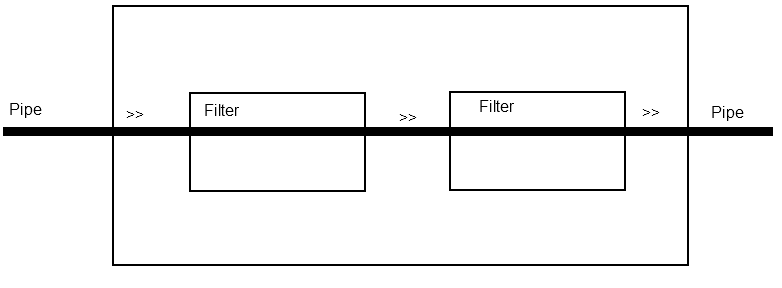
\includegraphics[width=\textwidth]{./planning/img/PipeAndFilter}
	\caption{Pipe and Filter Pattern\label{fig:pipefilter}}
\end{figure}

\subsection{Layered Architectural Pattern}
%-------------------------------------------------
\label{sec:Layered}
The layered architectural pattern is a pattern that involves grouping several different classes that all share the same dependencies. This grouping of classes is called a layer, and the layers are structured so that the classes inside each layer only depend on the classes of their own layer level, or inside an underlaying one. Structuring the code in this way helps delegating responsibilities to different parts of the system in a logical way, making the code easier to understand and easier to navigate through.

\autoref{fig:layered} shows how the layered architectural pattern is used in the \gls{utility}

\begin{figure}[htb]
	\center
	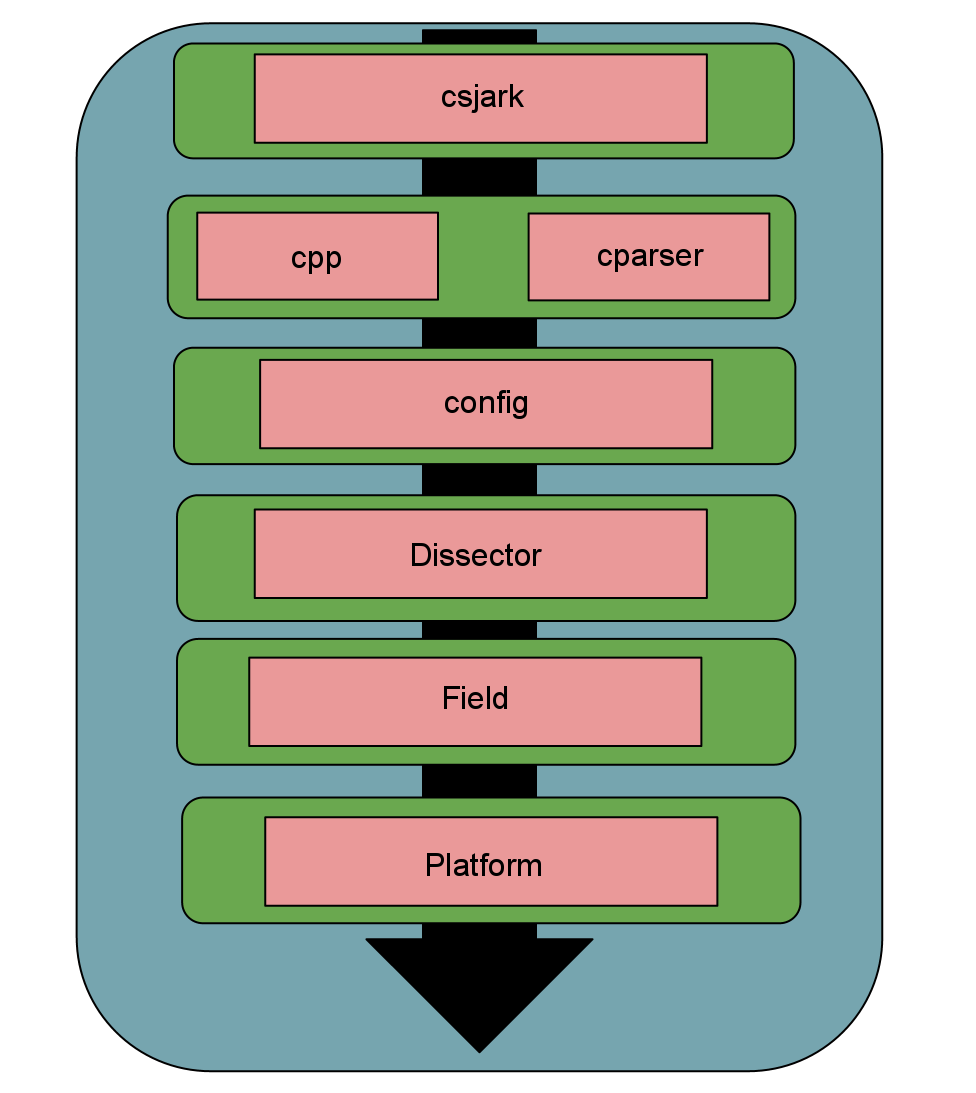
\includegraphics[width=0.7\textwidth]{./planning/img/layered}
	\caption{Layered Architectural Pattern in the \gls{utility}\label{fig:layered}}
\end{figure}

%----------------------------
\section{Architectural Views}
%----------------------------
This section describes three different views the team used for this project: A logical view, process view and a deployment view.

\subsection{Logical View}
%------------------------
\autoref{fig:logicalview} shows the logical view of the system.The command line takes the arguments for \gls{header} file and configuration file as a string. The arguments are parsed in the command line \gls{parser}. Header file is sent to ''\Gls{c} \gls{preprocessor} \& \Gls{c} \gls{parser}'', the \Gls{c} \gls{header} file is loaded and parsed by the \Gls{c} \gls{parser}, whcih generates a parsing tree. Command line also call Configuration, which load the configuration file. The configuration will parse the configuration file and create configuration rules. The \Gls{lua} \gls{script} generator will generate a \Gls{lua} \gls{script} from the parsing tree and the config rules.

\begin{figure}[htb]
	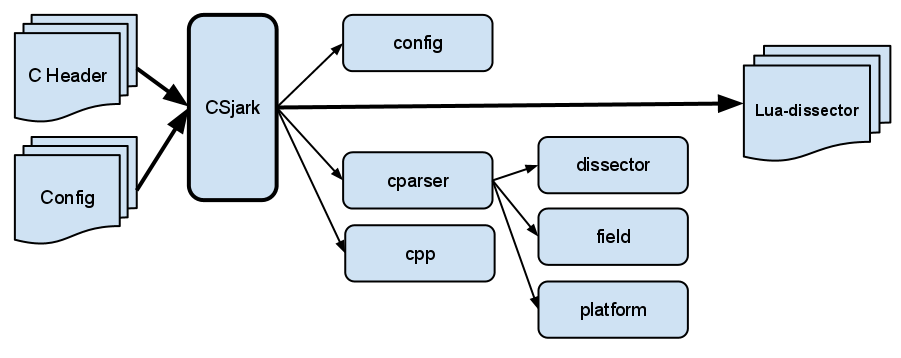
\includegraphics[width=\textwidth]{./planning/img/final_arch}
	\caption{Overall Architecture\label{fig:logicalview}}
\end{figure}

%---------------------
\subsection{Process View}
%---------------------
\autoref{fig:processview} shows the process view for our \gls{utility}. Csjark takes \gls{header} and config files as input and then uses the config and cparser to parse the files. CSjark then uses the cparser to find the \glspl{struct} in the \gls{header} file and then creates \glspl{dissector} for them. These \glspl{dissector} are then written to a file and CSjark then reports to the user by sending a message to the command line.

\begin{figure}[htb]
	\center
	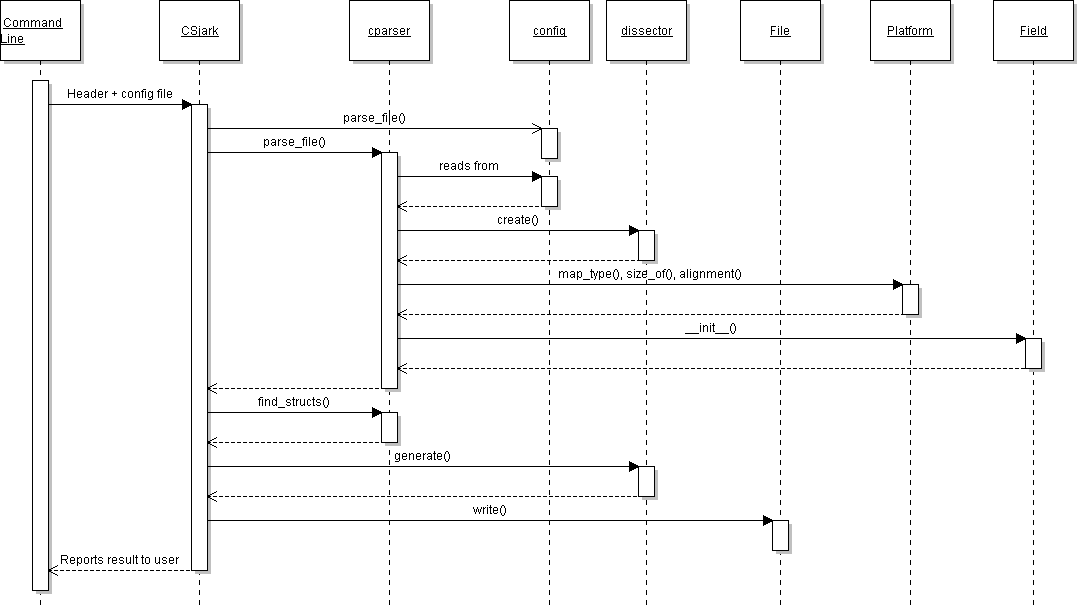
\includegraphics[width=\textwidth]{./evaluation/img/FinalSequenceDiagram}
	\caption{Data flow during regular execution\label{fig:processview}}
\end{figure}


%------------------------
\subsection{Deployment View}
%------------------------

\autoref{fig:deployment} shows the deployment diagram for this project. CSjark 
takes \gls{header}-files and config-files as input, and generates \Gls{lua} 
\glspl{dissector}. All these \glspl{dissector} are added as plugins to 
\Gls{wireshark}, extending the functionality. \Gls{wireshark} will capture the 
data packet when Process A send data to Process B, the \Gls{lua} 
\glspl{dissector} is used to display these data packets correctly.

\begin{figure}[htb]
	\center
	\includegraphics[width = 0.8\textwidth]{./planning/img/Deployment}
	\caption{Deployment View\label{fig:deployment}}
\end{figure}

%--------------------------------
\section{Architectural Rationale}
%--------------------------------
The team decided to use the pipe and filter pattern as the architects felt that it was one of the only architectural patterns that would benefit the \gls{utility} without having to make it needlessly complex. The \gls{utility} was supposed to take \gls{header} files as input and then process the data from them several times, until the end result was a list of \glspl{struct} and \glspl{member} that could be used to make \glspl{dissector} for \Gls{wireshark}. This seemed like an excellent application to use the pipe and filter pattern with, as it would then be easy to add new filters to the \gls{header} file for future increments of the development cycle without having to rewrite what had already been implemented in previous sprints.

The team also decided to use the layered architectural pattern as the code of the utility would have to stay logical and well structured through the entire project if we wanted the future development of the utility to go more smoothly. By dividing the entire utility into several modules and designate layers between them it became easier to decide which functionality would go where in the code which could save the different developers some grief. It would also make the code easier to inspect by whomever that wishes to understand the code and more specifically how the utility works.

For the views the team decided to use a logical view, process view and deployment view. These views were chosen because the architects of the \gls{utility} felt that these views alone could represent the system sufficiently without creating too much overhead for the readers of the document. The logical view supplies the reader with a more in depth view of what the system is comprised of, which is useful for developers who need to figure out the workings of the system. The process view also seemed important for the developers and the testers of the \gls{utility}, as it provides the reader with a more proper overview of the data flow in the system. This makes it a lot easier to see which modules are run when, and to see which external calls dictate the modules' behaviour. Lastly a deployment view was chosen to make it more clear for the reader of the document what the \gls{utility} really produces as output and what other external applications it has to cooperate with. 

